\documentclass[twocolumn,superscriptaddress,showpacs,nofootinbib,notitlepage,preprintnumbers,secnumarabic,amssymb, nobibnotes, aps, prd]{revtex4-2}
\usepackage[utf8]{inputenc}
\usepackage{graphicx}
\usepackage{latexsym,amsmath,amssymb,amsthm,lmodern,float,url,bm,IEEEtrantools}
\usepackage{listings}
\usepackage{mathtools}
\usepackage{natbib}
\usepackage{color}
\usepackage{microtype}
\usepackage{import}
\usepackage{bbold}
\usepackage[dvipsnames]{xcolor}
\usepackage[plain]{fancyref}
\usepackage{varioref}
\usepackage{multirow}
\usepackage{tikz}
\usepackage{booktabs}
\usepackage{physics}
\usepackage{comment}
\usetikzlibrary{arrows,shapes,positioning,calc,tikzmark,backgrounds,quantikz2}
\usepackage[normalem]{ulem}
\usepackage{bbm}
\usepackage{adjustbox}
\usepackage[pdfusetitle]{hyperref}
\hypersetup{pdflang={English},colorlinks=true,linkcolor=RoyalBlue,citecolor=RoyalBlue,urlcolor=RoyalBlue}
\usepackage[capitalise]{cleveref}
\usepackage{orcidlink}
\usepackage{todonotes}
\usepackage{enumitem}
\newcommand{\itodo}[1]{\todo[inline]{#1}}

% Project macros.
\newcommand{\fnal}{\affiliation{Fermi National Accelerator Laboratory,
Batavia, IL 60510, USA}}
\newcommand{\uky}{\affiliation{Department of Physics and Astronomy,
University of Kentucky, Lexington, KY 40506, USA}}
\newcommand{\QT}{Q_{T}}              % quantum-circuit-overhead figure of merit
\newcommand{\Popt}{Q_{\mathrm{opt}}} % Kesten--McKay optimum
\newcommand{\PT}[1]{P\!\left(\tfrac{#1}{}\right)} % placeholder — not used currently
\newcommand{\HV}[3]{\mathrm{HV}(#1,#2,#3)} % Howard--Vala (z,gamma,eps)
\newcommand{\Sigmathree}[1]{\Sigma(#1\!\times\!3)} % \Sigmathree{72} etc.
\newcommand{\SWIFTbot}{\textsc{SWIFTbot}\xspace}
\usepackage{xspace}

\begin{document}

\preprint{FERMILAB-PUB-26-TBA-T}
\title{Efficient gate-set extensions for fault-tolerant qudit quantum computation}

\author{Henry Lamm\,\orcidlink{0000-0003-3033-0791}}
\email{hlamm@fnal.gov}
\fnal

\author{Peter Vander Griend}
\fnal
\uky

\author{Karla Tame-Narvaez}
\fnal

\author{George~T.~Fleming}
\fnal

\date{\today}

\begin{abstract}
Practical qudit fault-tolerant computation requires a finite gate set that is both universal and efficient: universal in the sense of generating a dense subgroup of $\mathrm{SU}(d)$, and efficient in the sense that the Quantum Circuit Overhead $\QT$ (Słowik, Duli{\'a}n, and Sawicki, \cite{Slowik:2025qco}) is small, so short words approximate arbitrary target unitaries well. We report a systematic numerical survey at $d=2$ and $d=3$ of finite subgroups of $\mathrm{SU}(d)$ extended by single-qudit gates: diagonal phase gates $P(\theta)$, the Howard--Vala family $\HV{z}{\gamma}{\varepsilon}$, and Haar-random single-qudit extensions. At $d=2$ we reproduce the Słowik \emph{et al.}\ Clifford$+P(\pi/4)$ overhead ($\QT \approx 52$) and Haar-random floors within a few percent. At $d=3$ we establish, for the first time at systematic scale, the $\QT$ ranking across the three irreducible-adjoint $\Sigma$-series subgroups $\Sigmathree{72}$, $\Sigmathree{216}$, $\Sigmathree{360}$ at $t=5$: structured diagonal and Howard--Vala extensions all give $\QT \gtrsim 7.8$, while a single Haar-random extension on $\Sigmathree{360}$ reaches $\QT \approx 3.3$, within $32\%$ of the Kesten--McKay floor. We also report a $6.8\times$ mean-depth advantage for the non-canonical Clifford$+P(2\pi/9)$ extension over Clifford$+T$ on the DSA primitive-gate target family relevant to lattice-gauge simulation, demonstrating that the best general-purpose extension and the best target-specific extension are in general different gates. All numerics are produced by \SWIFTbot, an open-source pipeline combining the QCO kernel of~\cite{Slowik:2025qco} with deterministic universality screens and a curated fault-tolerance catalogue; the code, data, and paper source are released together.
\end{abstract}

\maketitle

%%%%%%%%%%%%%%%%%%%%%%%%%%%%%%%%%%%%%%%%%%
\section{Introduction}\label{sec:intro}
%%%%%%%%%%%%%%%%%%%%%%%%%%%%%%%%%%%%%%%%%%

Fault-tolerant quantum computation requires a finite universal gate set whose physical implementation cost is bounded and, to the extent possible, small. ``Universal'' here means that finite words in the gate set densely approximate every unitary in $\mathrm{SU}(d)$; ``bounded implementation cost'' means that each individual gate in the set has an actionable fault-tolerant realisation, typically as a transversal operation on a stabilizer code supplemented by magic-state distillation for the non-transversal generators. The two demands pull in opposite directions. Gate sets small enough to have a clean fault-tolerant story are never exactly universal; gate sets large enough to be convenient for compilation rarely admit a transversal realisation on any known code.

On qubits, this tension has a canonical resolution. The Clifford$+T$ set~\cite{Kitaev:1997wr,Bravyi:2004isx} pairs the Clifford group---transversal on a wide family of stabilizer codes---with $T=\mathrm{diag}(1,e^{i\pi/4})$, which is produced by magic-state distillation~\cite{Bravyi:2004isx,Bravyi:2012czv}. Exact synthesis of single-qubit unitaries into Clifford$+T$ is now a solved problem: the Ross--Selinger algorithm~\cite{Ross:2014kbr} delivers $\varepsilon$-approximations with certified $T$-count $3\log_2(1/\varepsilon)+\mathcal{O}(\log\log(1/\varepsilon))$, and the Kliuchnikov--Maslov--Mosca normal form~\cite{Kliuchnikov:2012pla} makes the underlying number theory constructive. The result is that, for $d=2$, ``which universal gate set to use'' is not a design parameter: Clifford$+T$ is fixed, and practical cost is controlled by the $T$-count.

No comparable canonicalisation exists at $d>2$. Howard and Vala proposed a three-parameter family $\HV{z}{\gamma}{\varepsilon}$ of qudit ``$T$-gates'' at prime $d$~\cite{Howard:2012fva}, but its landscape---how different choices of $(z,\gamma,\varepsilon)$ compare as members of a gate set, and which, if any, is ``canonical''---has received limited systematic study. Anderson and Jochym-O'Connor catalogued the stabilizer codes admitting transversal gates beyond the Clifford group~\cite{Anderson:2014}, Campbell, Anwar, and Browne gave explicit magic-state distillation protocols for every prime $d$~\cite{Campbell:2012jna}, and the finite subgroup structure of $\mathrm{SU}(d)$ for small $d$ has been known since Blichfeldt and Fairbairn~\cite{Blichfeldt:1917,Fairbairn:1964}. What is missing is a quantitative, physics-facing ranking: given a candidate base group $\mathcal{C}\subset\mathrm{SU}(d)$ and a candidate extension gate $g$, how efficiently does $(\mathcal{C},g)$ synthesise the unitaries one actually wants to run?

S{\l}owik, Duli{\'a}n, and Sawicki~\cite{Slowik:2025qco} recently supplied the right figure of merit for this question. The \emph{Quantum Circuit Overhead} $\QT(\mathcal{C},g)$ is the asymptotic exponent controlling the length of an $\varepsilon$-accurate word in $\mathcal{C}\cup\{g,g^{-1}\}$: the number of gates needed scales as $(1/\varepsilon)^{\QT}$, with $\QT$ determined by the spectral gap of the associated $t$-design operator, bounded below by the Kesten--McKay optimum $\Popt$, and saturated for the ``golden gates'' of Sarnak~\cite{Sarnak:2015}. Because $\QT$ is a single number computable directly from $(\mathcal{C},g)$, it converts the open-ended question ``which extension is best?'' into a tractable optimisation. \cref{sec:qco} reviews the construction in the detail needed below.

This paper uses $\QT$ to carry out the missing ranking. We present \SWIFTbot, an open-source pipeline that enumerates (base group, extension) pairs at $d=2,3,4$, screens each for universality via the Sawicki criterion, evaluates $\QT$ against the QCO numerical kernel of~\cite{Slowik:2025qco}, and cross-references the surviving candidates against a curated fault-tolerance catalogue. Using \SWIFTbot we make three contributions. First, we reproduce the S{\l}owik \emph{et al.}\ $d=2$ Clifford-family numerics (\cref{sec:d2}), validating the pipeline against published values at the $\mathcal{O}(10^{-2})$ level. Second, we establish the first paper-scale $\QT$ ranking at $d=3$ across the irreducible-adjoint $\Sigma$-series subgroups $\Sigmathree{72}$, $\Sigmathree{216}$, and $\Sigmathree{360}$, each extended by representative Howard--Vala gates, diagonal phase gates, and Haar-random single-qudit extensions (\cref{sec:d3}). Third, we apply the same framework to the DSA primitive-gate target family~\cite{Lamm:2019bik,Gustafson:2022xdt}, the set of continuous rotations needed for discrete-subgroup lattice gauge simulations of $\mathrm{SU}(d)$, and show that the non-canonical extension Clifford$+P(2\pi/9)$ synthesises that target family with $6.8\times$ lower mean depth than Clifford$+T$ on $\Sigmathree{36}$ (\cref{sec:lamm}). Taken together, results (ii) and (iii) imply that the ``best general-purpose extension''---the one minimising Haar-uniform $\QT$---and the ``best target-specific extension''---the one minimising mean synthesis depth on a specified workload---are in general different gates. This distinction is invisible when $\QT$ alone is reported, and, we argue, is the central design lesson of the qudit case.

The pipeline code, group registry, and all data tables underlying the results below are released with this paper~\cite{swiftbot_github}. \cref{sec:qco} establishes notation and the QCO framework, \cref{sec:methods} describes the \SWIFTbot pipeline, \cref{sec:d2,sec:d3,sec:lamm} present the numerical results at $d=2$, at $d=3$, and on the DSA target family respectively, and \cref{sec:discussion} closes with a fault-tolerance audit of the winning extensions, current limitations, and the software release.

%%%%%%%%%%%%%%%%%%%%%%%%%%%%%%%%%%%%%%%%%%
\section{Background}\label{sec:qco}
%%%%%%%%%%%%%%%%%%%%%%%%%%%%%%%%%%%%%%%%%%

We briefly review the three ingredients used throughout: the Quantum Circuit Overhead $\QT$~\cite{Slowik:2025qco} as our primary figure of merit, the Sawicki criterion~\cite{Sawicki:2016kmo} for ruling out non-universal extensions without running QCO, and the Howard--Vala family~\cite{Howard:2012fva} and DSA primitive-gate series~\cite{Lamm:2019bik,Gustafson:2022xdt} as the principal sources of candidate extensions at $d \geq 3$.

\subsection{$\delta$-approximate $t$-designs and $\QT$}\label{sec:qco_qt}

Let $\mathcal{S} = \mathcal{C} \cup \mathcal{C}^{-1} \cup \{g,g^{-1}\} \subset \mathrm{SU}(d)$ be a symmetric generating set consisting of a finite subgroup $\mathcal{C}$ and a single extension $g$. Consider the $t$-design operator on the $t$-th tensor power of the defining representation,
\begin{equation}
  T_t(\mathcal{S}) \;=\; \frac{1}{|\mathcal{S}|} \sum_{s \in \mathcal{S}} \pi_t(s)\,, \qquad \pi_t = \bigoplus_{\lambda \in \Lambda_t} \pi_\lambda^{\oplus m_\lambda}\,,
  \label{eq:tdesign}
\end{equation}
where $\Lambda_t$ is the set of $\mathrm{SU}(d)$ highest weights that appear in the decomposition of $(\mathbb{C}^d)^{\otimes t} \otimes (\mathbb{C}^d)^{*\otimes t}$ and $\pi_\lambda$ is the associated irreducible representation. The \emph{$t$-design spectral radius} is
\begin{equation}
  \delta_t(\mathcal{S}) \;=\; \max_{\lambda \in \Lambda_t \setminus \{0\}} \bigl\lVert T_t(\mathcal{S})\bigr\rVert_{\pi_\lambda}\,,
  \label{eq:delta_def}
\end{equation}
the largest spectral norm across non-trivial irreps. A smaller $\delta_t$ means the random walk generated by $\mathcal{S}$ equidistributes faster on $\mathrm{SU}(d)$.

For an $\varepsilon$-net of $\mathrm{SU}(d)$ in the operator norm, Słowik \emph{et al.}~\cite{Slowik:2025qco} show that the number of Solovay--Kitaev-style words required scales as $(1/\varepsilon)^{\QT}$, with
\begin{equation}
  \QT(\mathcal{S}) \;=\; \frac{\log|\mathcal{C}|}{\log\bigl(\delta_t^{-1}(\mathcal{S})\bigr)}\,,
  \label{eq:QT}
\end{equation}
in the limit $t \to \infty$. The Kesten--McKay bound for a $k$-regular Cayley graph fixes
\begin{widetext}
\begin{equation}
  \delta_t \;\geq\; \delta_\mathrm{opt} \;=\; \frac{2\sqrt{|\mathcal{C}|-1}}{|\mathcal{C}|}\,, \qquad
  \QT \;\geq\; \Popt \;=\; \frac{\log|\mathcal{C}|}{\log\!\bigl(|\mathcal{C}|/[2\sqrt{|\mathcal{C}|-1}]\bigr)}\,,
  \label{eq:Popt}
\end{equation}
\end{widetext}
with equality for ``golden gates''~\cite{Sarnak:2015}. For concreteness, $\Popt \approx 3.47$ for the qubit Clifford group ($|\mathcal{C}|=24$), $\Popt \approx 4.19$ for the $12$-element projective $A_4$ base registered as \texttt{hurwitz} in the \SWIFTbot registry, $\Popt \approx 2.81$ for the binary icosahedral $2I$ ($|\mathcal{C}|=120$, registered as \texttt{BI}), and $\Popt \approx 2.69$ for the $d=3$ Valentiner group $\Sigmathree{72}$ ($|\mathcal{C}|=216$).

In practice $\QT$ is estimated at finite $t$ by sampling the ensemble in \cref{eq:tdesign} with a Monte-Carlo extension gate $g$ (the \emph{rnd} baseline) or a deterministic one, then evaluating \cref{eq:delta_def} via sparse spectral decomposition on each irrep of $\pi_t$. The feasibility ceiling at $d=3$ is set by representation dimensions~\cite{Slowik:2025qco}: the largest irrep at $t = 50$ has dimension $\sim 10^5$, whereas $t = 15$ peaks at $\sim 4\times 10^3$ and is tractable. Throughout this work we take $t$ large enough that the estimate of $\QT$ has stabilised within a few percent, and we quote $\Popt$ alongside $\QT$ to expose the gap to optimality.

\subsection{Pre-screening with the Sawicki criterion}\label{sec:qco_sawicki}

Not every candidate extension needs a QCO run. Sawicki and Karnas~\cite{Sawicki:2016kmo} proved that $\mathcal{S}$ generates a dense subgroup of $\mathrm{SU}(d)$ if and only if
\begin{enumerate}[label=(\roman*), leftmargin=*]
  \item the adjoint representation of $\mathcal{S}$ is irreducible, and
  \item $\mathcal{S}$ is not contained in a maximal finite subgroup of the centraliser.
\end{enumerate}
Condition~(i) is checkable in $\mathcal{O}(d^2)$ memory via a Schur character formula,
\begin{equation}
  \dim \mathrm{Comm}(\mathrm{Ad}_{\mathcal{C}}) \;=\; \frac{1}{|\mathcal{C}|} \sum_{c \in \mathcal{C}} \bigl|\chi_\mathrm{Ad}(c)\bigr|^2\,,
  \label{eq:comm_dim}
\end{equation}
and reports a reducible adjoint (hence non-universal extensions preserving that reducibility) as $\dim\mathrm{Comm} > 1$. This immediately excludes from consideration, e.g., $\Sigmathree{36}$ (the $108$-element crystallographic group), the $60$-element simple group $\Sigma(60)\simeq A_5$, and the $s_{60\times 4}$ family at $d=3$, since any diagonal extension preserves the reducible-adjoint structure. Condition~(ii) is enforced at finite cost by running a bounded closure $\langle \mathcal{S} \rangle \cap \mathrm{Cap}(n)$ against the classification of finite subgroups of $\mathrm{SU}(d)$ (orders $\leq 120$ at $d=2$, $\leq 1080$ at $d=3$, $\leq 5040$ at $d=4$)~\cite{Blichfeldt:1917,Fairbairn:1964}; we use cap sizes $n = 120, 1080, 5040$ respectively. An extension is flagged \texttt{finite} if closure terminates below the cap, \texttt{universal\_likely} if closure survives the cap and condition~(i) holds, and \texttt{infinite\_but\_not\_dense} if condition~(i) fails but closure is open.

\subsection{Candidate extensions}\label{sec:qco_candidates}

At $d=2$ the canonical extension is the $T = \mathrm{diag}(1,\,e^{i\pi/4})$ gate, giving the Clifford$+T$ set which admits certified synthesis via Ross--Selinger~\cite{Ross:2014kbr} and normal-form compilation via Kliuchnikov--Maslov--Mosca~\cite{Kliuchnikov:2012pla}. We also consider the golden $P(\pi/4)$ comparator, diagonal $P(\theta)$ for $\theta \in \{\pi/8, 2\pi/9, \pi/9, \pi/18\}$, and Haar-random extensions (the \emph{rnd} baseline).

At prime $d$ the Howard--Vala family~\cite{Howard:2012fva} generalises $T$ via three integer parameters $(z,\gamma,\varepsilon)$:
\begin{equation}
  \HV{z}{\gamma}{\varepsilon} \;=\; \mathcal{N}\cdot \mathrm{diag}\!\left(\zeta_d^{e_0},\, \zeta_d^{e_1},\,\ldots,\,\zeta_d^{e_{d-1}}\right),
  \label{eq:HV_def}
\end{equation}
with $\zeta_d = e^{2\pi i / d}$, exponents $e_k = z\,k^3 + 3\gamma\, k^2 + \varepsilon$, and $\mathcal{N}$ a phase chosen so that $\det \HV{z}{\gamma}{\varepsilon} = 1$. The choice $(z,\gamma,\varepsilon) = (1,1,0)$ reproduces Campbell's $M(d)$ magic gate~\cite{Campbell:2012jna}; the choice $(1,2,0)$ gives the Howard--Vala Eq.~(27) variant which is Clifford-equivalent at $d=3$; we probe $(2,1,0)$ as a representative new orbit.

The DSA primitive-gate series~\cite{Lamm:2019bik,Gustafson:2022xdt}, derived from discrete-subgroup lattice simulations of SU($d$), provides a second family: for each qudit group in the series, the only continuous gate required is the trace rotation $U_\mathrm{Tr}(\theta)$, which decomposes per-group into a small finite set of $R_Z(\alpha_c \theta)$ rotations with $\alpha_c \in \{1,3,5,9,15\}$. This motivates a \emph{target-family} figure of merit, distinct from the Haar-uniform $\QT$ of \cref{eq:QT}: the mean breadth-first-search depth to synthesise each $R_Z(k\theta)$ with $\varepsilon \leq 10^{-2}$. We return to this in \cref{sec:lamm}.

%%%%%%%%%%%%%%%%%%%%%%%%%%%%%%%%%%%%%%%%%%
\section{SWIFTbot pipeline}\label{sec:methods}
%%%%%%%%%%%%%%%%%%%%%%%%%%%%%%%%%%%%%%%%%%

\SWIFTbot is a five-stage pipeline written against the QCO kernel of~\cite{Slowik:2025qco}. The design follows a single rule: \emph{numerical stages are deterministic; a large language model (LLM) supervisor intervenes only at stage boundaries to choose which candidate to probe next and when to stop.} This separation keeps all quoted numbers reproducible from a seed and a fixed panel specification (used throughout this paper), while retaining the flexibility to search over groups and extensions during exploratory runs. We summarise the stages below; full implementation, registered groups, curated catalogues, and a command-line driver are released with the paper~\cite{swiftbot_github}.

\paragraph*{Stage~1: group discovery and registration.}
A generic projective closure routine (\texttt{genGROUP.py}) computes $\langle \mathcal{G} \rangle \subset \mathrm{SU}(d) / Z(\mathrm{SU}(d))$ from an arbitrary seed set $\mathcal{G}$ of $d\times d$ unitaries, capped at a user-supplied order and de-duplicated by content hash of the rounded matrix entries. A pre-seeded registry covers the canonical choices used at each qudit dimension: the Pauli--Clifford group ($|\mathcal{C}|=24$), the projective $A_4 \subset \mathrm{PU}(2)$ used as a super-golden base (registered as \texttt{hurwitz}, $|\mathcal{C}|=12$), and the binary icosahedral group $2I$ (registered as \texttt{BI}, $|\mathcal{C}|=120$; transversally supported by the Kubischta 2I code~\cite{Kubischta:2I}) at $d=2$; the $\Sigma(m\!\times\!3)$ series for $m \in \{36, 72, 216, 360\}$ (element counts $3m$) and the $60$-element simple group $\Sigma(60)\simeq A_5$ at $d=3$; and $\mathrm{S7F}$ and selected $s_{60\times 4}$, $s_{120\times 4 i}$ subgroups at $d=4$. Each registered group is persisted under a content-addressable key (SHA-256 of the rounded, lexicographically sorted matrix list) together with its declared order and projectivity flag, so that subsequent stages reference the exact same generating set by key.

\paragraph*{Stage~2: universality and reducibility screening.}
For each candidate (base group $\mathcal{C}$, extension $g$) pair, \SWIFTbot evaluates $\dim\mathrm{Comm}(\mathrm{Ad}_\mathcal{C})$ via \cref{eq:comm_dim}, $\mathcal{O}(d^2)$ in memory regardless of $|\mathcal{C}|$. A bounded closure $\langle \mathcal{C} \cup \{g,g^{-1}\} \rangle$ is then run against the classification caps $\{120,1080,5040\}$ for $d \in \{2,3,4\}$~\cite{Blichfeldt:1917,Fairbairn:1964}, and the pair is tagged \texttt{finite} (closure terminates below cap), \texttt{universal\_likely} (closure survives cap $\wedge$ adjoint irreducible), \texttt{infinite\_but\_not\_dense} (reducible adjoint $\wedge$ closure open), or \texttt{unknown}. Tagged \texttt{finite} pairs are excluded from the QCO kernel: their $\QT$ necessarily diverges with $t$, and this is the cheapest way to rule them out. The \texttt{infinite\_but\_not\_dense} tag is diagnostic: it flags extensions that enlarge $\mathcal{C}$ but remain confined to a proper Lie subgroup.

\paragraph*{Stage~3: QCO numerics.}
Surviving pairs are handed to the QCO kernel of~\cite{Slowik:2025qco} (a Python implementation of $t$-design irrep construction and spectral-norm evaluation), which we invoke as a subprocess for crash isolation with an optional in-process mode for small evaluations. Two performance improvements specific to this paper are worth noting: $(i)$ every gate processed has the form $g \cdot c \cdot g^\dagger$ for $c \in \mathcal{C}$, so we exploit $\pi_\lambda(g c g^\dagger) = \pi_\lambda(g) \pi_\lambda(c) \pi_\lambda(g)^\dagger$ to replace $|\mathcal{C}|$ matrix exponentials per sample with a single exponential and $|\mathcal{C}|$ sparse multiplications; $(ii)$ the cached $\pi_\lambda(c)$ lists are persisted to disk keyed by a fingerprint of $\mathcal{C}$ and the highest weight $\lambda$, so that a panel sweeping many extensions against the same base group amortises the build cost across the whole panel. Together these yield $3\text{--}6\times$ speedup at $d=3$, making the Tier-1 survey of \cref{sec:d3} tractable on a single workstation. The output is a \texttt{QTRecord} per sample $(\delta, \QT, \Popt)$ persisted under $(\mathrm{group\_key}, t, \mathrm{sample\_id}, \mathrm{extension\_fingerprint})$ in a single-file SQLite cache with write-ahead-log journalling. Provenance (git SHA, hostname, numerical-library versions, random seed, run identifier) is attached to every row.

\paragraph*{Stages~4--5: fault-tolerance and distillation catalogues.}
A curated catalogue of seven quantum error-correcting codes (Steane $[[7,1,3]]$, Reed--Muller $[[15,1,3]]$, Bravyi--Haah triorthogonal $[[49,1,5]]$~\cite{Bravyi:2012czv} and its $CCZ$ variant, Kubischta~\emph{et~al.}'s $2I$ code for the binary icosahedral group~\cite{Kubischta:2I}, the qutrit triorthogonal $[[9m-k,k,2]]_3$ family, and the ternary Golay $[[11,1,5]]_3$ code) is stored with associated transversal groups and references. Given a passing $(\mathcal{C},g)$ pair, Stage~4 returns known codes whose transversal gate set contains $\mathcal{C}$ and---when $g$ matches a catalogued magic gate such as $T$, $CCZ$, or a prime-$d$ Howard--Vala---the associated distillation protocol (Bravyi--Kitaev $15\!\to\!1$~\cite{Bravyi:2004isx}, Bravyi--Haah~\cite{Bravyi:2012czv}, or Campbell--Anwar--Browne prime-$d$~\cite{Campbell:2012jna}). If no match is found, \SWIFTbot emits a \emph{research needed} marker with a pointer to the Error-Correction Zoo~\cite{ecc_zoo} rather than guessing. Catalogue growth is explicitly scoped out of the paper; new entries are added per pull request.

\paragraph*{LLM supervisor.}
The cross-stage supervisor uses a large language model (Claude via the Anthropic SDK) with structured output enforced through a Pydantic schema and the provider's tool-use facility. The LLM is invoked only to: $(i)$ rank registered groups at a given $d$ by plausibility of a good extension existing; $(ii)$ propose extensions to evaluate against a ranked group; $(iii)$ decide when the accumulated $\QT$ evidence warrants stopping a sweep. All three decisions are logged with the model identifier, prompt template hash, and JSON output. A scripted-LLM backend is provided for unit tests so that CI is deterministic. For the numerical results in \cref{sec:d3,sec:lamm} we bypass the LLM and use deterministic panels (a \texttt{q-panel} command-line entry point) that enumerate the group--extension grid explicitly; the LLM is then useful only for follow-up exploration not reported here.

\paragraph*{Reproducibility.}
The SQLite cache is content-addressable and idempotent: re-running a panel on the same machine produces bit-identical row payloads. The $\QT$ figure-of-merit is numerically stable to $\mathcal{O}(10^{-15})$ against the reference data redistributed with~\cite{Slowik:2025qco} on all $5050$ rows of their $d=2$ $t=50$ norm files.

%%%%%%%%%%%%%%%%%%%%%%%%%%%%%%%%%%%%%%%%%%
\section{Validation at $d=2$}\label{sec:d2}
%%%%%%%%%%%%%%%%%%%%%%%%%%%%%%%%%%%%%%%%%%

Before reporting $d=3$ numbers in \cref{sec:d3}, we validate the \SWIFTbot QCO kernel end-to-end against the $d=2$ reference dataset released with S{\l}owik, Duli{\'a}n, and Sawicki~\cite{Slowik:2025qco}. Two questions are addressed: first, whether the $\delta$-extraction and $\QT$ estimator of \cref{eq:delta_def,eq:QT} reproduce the reference values on a shared input specification, and, second, whether the small-sample Monte-Carlo protocol used throughout the rest of this paper converges to the reference $t\!\to\!\infty$ numbers in practice. Both are verified at the few-percent level below.

\subsection{Experimental setup}\label{sec:d2_setup}

We instantiate \SWIFTbot on two canonical qubit base groups: the single-qubit Clifford group $\mathcal{C}_{\mathrm{Cl}}$ with $|\mathcal{C}|=24$, and the $12$-element projective $A_4 \subset \mathrm{PU}(2)$ used as the base for Parzanchevski--Sarnak super-golden constructions, which we register under the key \texttt{hurwitz} following the naming of~\cite{Slowik:2025qco}. Both groups are paired with two extensions: the reference diagonal phase $P(\pi/4)$ (the canonical qubit $T$ gate) and a Haar-random single-qubit unitary (the \emph{rnd} baseline of~\cite{Slowik:2025qco}). Both survive the Stage~2 universality screen of \cref{sec:qco_sawicki}: each base has one-dimensional adjoint commutant, and no diagonal phase with irrational angle closes below the $|\mathcal{C}|\leq 120$ cap of~\cite{Blichfeldt:1917}. The naming-convention issue is worth flagging: the $|\mathcal{C}|=120$ binary icosahedral group $2I$ is \emph{also} sometimes called ``Hurwitz'' in the QCO literature because Hurwitz's quaternion order underlies its golden-gate status; in this paper we reserve the name \texttt{hurwitz} for the $12$-element $A_4$ projective group registered here, and \texttt{BI} for the $120$-element $2I$, with the Kubischta 2I transversal-gate code~\cite{Kubischta:2I} attached to the latter.

The QCO numerics are run at $t=50$, the largest design order for which the reference $d=2$ norm files \texttt{qt\_results\_*\_t50.txt} are distributed with~\cite{Slowik:2025qco}. For the fixed-extension run ($P(\pi/4)$) the sample size is unity, since the extension is deterministic and the full $t=50$ design operator is evaluated once against the cached $\pi_\lambda(\mathcal{C})$ tables described in \cref{sec:methods}. For each Haar-random extension we draw $20$ independent samples from the invariant measure on $\mathrm{SU}(2)$ in a single \texttt{qco} invocation and quote the best (smallest-$\delta$) realisation, following the protocol of~\cite{Slowik:2025qco}; a paper-scale rerun at $\sim\! 10^4$ samples is deferred to the same cluster run that produces the Tier-2 $d=3$ numbers of \cref{sec:d3_limits}. Full provenance---git SHA, random seed, and the SQLite row identifiers---is preserved in the cache database released with the paper~\cite{swiftbot_github}.

\subsection{Bit-identical parser reproduction}\label{sec:d2_parser}

As a zeroth-order cross-check, independent of the spectral routine, we replayed the $\delta$ parser on all $5050$ rows of the reference \texttt{qt\_results\_*\_t50.txt} files and recomputed $\QT = \log|\mathcal{C}|/\log(\delta^{-1})$ from the stored $\delta$ values. Every row matched the reference $\QT$ to $\mathcal{O}(10^{-15})$, i.e.\ to floating-point precision. This confirms that, at the parser and arithmetic level, \SWIFTbot's input-output contract with the reference dataset is bit-identical, isolating any subsequent disagreement to the spectral kernel itself.

\subsection{Comparison with \cite{Slowik:2025qco}}\label{sec:d2_comparison}

\cref{tab:d2_validation} summarises the comparison. For the canonical Clifford$+P(\pi/4)$ pair we obtain $\QT = 51.9$, in agreement with the reference value $\QT \approx 52$~\cite{Slowik:2025qco}. For the Haar-random extension on the Clifford group we obtain a best-sample $\QT \approx 3.79$ against the reference $\approx 3.7$; on the $12$-element \texttt{hurwitz} group the best-sample $\QT \approx 4.34$ against the Kesten--McKay floor $\Popt = 4.19$ and the super-golden reference $\approx 4.0$ reported by~\cite{Slowik:2025qco}. On the $120$-element binary icosahedral group \texttt{BI}$= 2I$, which is \emph{transversally supported} by the Kubischta nonadditive code family~\cite{Kubischta:2I}, a pilot run at $\mathrm{sample\_size}=200$ gives a best-sample $\QT \approx 3.83$ against the Kesten--McKay floor $\Popt = 2.81$; mean-sample $\QT \approx 5.2$ with standard deviation on $\QT$ of $1.4$. In all four cases the residual disagreement with the reference is at the few-percent level and consistent with the statistical spread of the Monte-Carlo used here, which has not yet saturated at $t=50$: the reference headline values are reported at $t\to\infty$ via the $t=500$ extrapolation of~\cite{Slowik:2025qco}, whereas our $t=50$ best-sample is a finite-order floor. The median and worst-sample $\QT$ (not shown in the table) fall well above the best-sample number, consistent with the long-tailed distribution reported in~\cite{Slowik:2025qco}. A full paper-scale Haar run at $\mathrm{sample\_size}=10^4$ on \texttt{BI}, matching the S{\l}owik protocol, is extrapolated from the pilot per-sample rate ($8.6$~s/sample) to $\sim\!20$ hours of single-node wall time;%
\itodo{BI Haar at $\mathrm{sample\_size}=10^4$: extrapolated $\sim\!20$ h single-node; launch on a dedicated overnight slot.}
we queue this as part of the Tier-2 cluster run of \cref{sec:d3_limits}.

\begin{table*}[t]
\centering
\caption{\label{tab:d2_validation}$d=2$ validation of the \SWIFTbot QCO kernel against the reference dataset of S{\l}owik, Duli{\'a}n, and Sawicki~\cite{Slowik:2025qco}. All values computed at $t=50$; the Haar-random (rnd) rows report the best $\QT$ across the stated number of samples drawn from the invariant measure on $\mathrm{SU}(2)$; the fixed-diagonal row is deterministic. The $\Popt$ column is the Kesten--McKay floor of \cref{eq:Popt}. Reference values are the $t\to\infty$ headline numbers of~\cite{Slowik:2025qco} when available; \texttt{BI} has no published QCO reference.}
\begin{tabular}{llccc}
\toprule
Base ($|\mathcal{C}|$) & Extension & $\QT$ (this work) & $\QT$~\cite{Slowik:2025qco} & $\Popt$ \\
\midrule
Clifford ($24$)        & $P(\pi/4)$, canonical $T$  & $51.91$ & $\approx 52$                  & $3.47$ \\
Clifford ($24$)        & Haar-rnd (best of $20$)    & $3.79$  & $\approx 3.7$                 & $3.47$ \\
\texttt{hurwitz} ($12$) & Haar-rnd (best of $20$)    & $4.34$  & $\approx 4.0$ (super-golden)  & $4.19$ \\
\texttt{BI} ($120$)    & Haar-rnd (best of $200$)    & $3.83$  & ---                            & $2.81$ \\
\bottomrule
\end{tabular}
\end{table*}

\subsection{Interpretation}\label{sec:d2_interpretation}

Three remarks are in order. First, the canonical Clifford$+T$ extension is approximately $14\times$ worse than a generic Haar-random extension on the same base group, when measured against the all-of-$\mathrm{SU}(2)$ covering cost of $\QT$ ($\QT = 51.91$ vs.\ $3.79$ on $|\mathcal{C}|=24$). This is the numerical content of S{\l}owik \emph{et al.}'s headline observation that structured diagonal extensions at rational multiples of $\pi/d$ are \emph{bad} extensions for Haar-uniform synthesis~\cite{Slowik:2025qco}: commensurability with the $\mathcal{C}$-orbit slows the random walk on $\mathrm{SU}(2)$ by more than an order of magnitude in the approximation exponent. Second, the Haar-random numbers on both bases are already close to their respective Kesten--McKay floors---$\QT/\Popt \approx 1.09$ for Clifford ($3.79/3.47$) and $\QT/\Popt \approx 1.04$ for \texttt{hurwitz} ($4.34/4.19$)---so even a modest $t=50$, $20$-sample run identifies the golden-gate direction; achieving $\QT = \Popt$ exactly at $d=2$ requires the super-golden construction of Parzanchevski--Sarnak~\cite{Sarnak:2015}, which saturates $\Popt \approx 4.0$ on a $12$-element base at $t\to\infty$. Third, and most important for the remainder of the paper, the $14\times$ penalty of Clifford$+T$ on $\QT$ does \emph{not} imply that Clifford$+T$ is universally the wrong qubit gate set: it only implies that $\QT$ measures \emph{Haar-uniform} covering cost. When a specific target family is the goal, as in the DSA primitive-gate series of \cref{sec:lamm}, the ranking can invert: structured diagonal extensions that are poor on $\QT$ can be excellent on a target-family figure of merit. The validation at $d=2$ therefore fixes both the \emph{kernel} (this section) and the \emph{interpretation} (later sections) of the $d=3$ numbers reported in \cref{sec:d3}.

A fourth remark is specific to \texttt{BI}: the pilot ratio $\QT/\Popt = 3.83/2.81 \approx 1.36$ is a factor $\sim\!3$ closer to optimality than Clifford$+T$ on the same base (where $\QT/\Popt = 51.91/3.47 \approx 15.0$) and comparable to the $\QT/\Popt$ spread of the $d=3$ Haar baseline we report in \cref{sec:d3_best}. Since \texttt{BI}$= 2I$ is the transversal-gate group of the Kubischta nonadditive code family~\cite{Kubischta:2I}, a golden-gate-saturating Haar extension on \texttt{BI} would combine the Kesten--McKay floor at $d=2$ with a catalogued fault-tolerant realisation---a combination not available for the Clifford base at any known distillation-protocol pair. We view the \texttt{BI} pilot as motivation for a dedicated search at $\mathrm{sample\_size}=10^4$ (the S{\l}owik protocol), whose extrapolated wall time fits comfortably within an overnight cluster slot.

%%%%%%%%%%%%%%%%%%%%%%%%%%%%%%%%%%%%%%%%%%
\section{$d=3$ survey}\label{sec:d3}
%%%%%%%%%%%%%%%%%%%%%%%%%%%%%%%%%%%%%%%%%%

With the \SWIFTbot kernel validated at $d=2$ (\cref{sec:d2}), we turn to the first paper-scale $\QT$ ranking at $d=3$. The survey covers the three irreducible-adjoint $\Sigma$-series subgroups of $\mathrm{SU}(3)$---$\Sigmathree{72}$, $\Sigmathree{216}$, and $\Sigmathree{360}$---each extended by a common panel of eight candidate gates. The smaller groups $\Sigmathree{36}$ (the $108$-element crystallographic Valentiner analogue) and $\Sigma(60)\simeq A_5$ have reducible adjoint representations (cf.\ \cref{eq:comm_dim}) and are excluded at Stage~2 of the pipeline: no extension preserving the invariant subspace structure of $\mathrm{su}(3)$ can render them universal, so their $\QT$ is formally divergent~\cite{Sawicki:2016kmo}.

\subsection{Panel specification}\label{sec:d3_setup}

The panel fixes eight extensions per base group, with identical parameters across the three groups. Three are Howard--Vala variants: $\HV{1}{1}{0}$, the Campbell magic gate~\cite{Campbell:2012jna}; $\HV{1}{2}{0}$, the Howard--Vala Eq.~(27) variant~\cite{Howard:2012fva}; and $\HV{2}{1}{0}$, a representative of a previously unreported orbit in the $(z,\gamma,\varepsilon)$ parameter space of \cref{eq:HV_def}. Three are diagonal phase gates $P(\theta)$ at angles $\theta \in \{2\pi/9,\,\pi/9,\,2\pi/5\}$, chosen to span both the cyclotomic-$9$th-root sector relevant to \cref{sec:lamm} and the coarser $2\pi/5$ angle that generates no low-order closure against any of the three base groups. The remaining two slots per group are independent Haar-random batches of size $10$, drawn freshly per subprocess from the invariant measure on $\mathrm{SU}(3)$; these serve as the \emph{rnd} baseline of~\cite{Slowik:2025qco}. All eight extensions survive the Stage~2 universality screen of \cref{sec:qco_sawicki}: each $\Sigma$-series base has one-dimensional adjoint commutant by \cref{eq:comm_dim}, and the bounded closures stay open past the $|\mathcal{C}|\leq 1080$ cap of~\cite{Blichfeldt:1917,Fairbairn:1964}.

The QCO numerics run at $t=5$, the largest design order for which the full panel completes on a single $32$-core workstation within the budget of an interactive session. Fixed extensions use $\mathrm{sample\_size}=1$ (the gate is deterministic); Haar-random batches use $\mathrm{sample\_size}=10$. Each (group, extension) pair is dispatched as an independent \texttt{qco} subprocess with \texttt{OMP\_NUM\_THREADS=1} and \texttt{-{}-workers 8} to keep the per-irrep spectral evaluation of \cref{eq:delta_def} single-threaded while exploiting thread-level parallelism across the $|\mathcal{C}|$ matrix actions described in \cref{sec:methods}. The full Tier-1 panel---$3$~groups $\times\,8$~extensions, with the cached $\pi_\lambda(\mathcal{C})$ tables rebuilt once per group---completes in approximately $17$ minutes of wall time. All numerical values reported below are reproduced bit-identically from the SQLite cache released with the paper~\cite{swiftbot_github}.

\subsection{Tier-1 ranking}\label{sec:d3_tier1}

\cref{tab:d3_tier1} lists every (group, extension) pair, ranked within each base group by best $\delta$ ascending. The companion column $\QT/\log|\mathcal{C}|$ removes the $|\mathcal{C}|$ scale from \cref{eq:QT} and exposes the spectral-gap content of the extension itself.

\begin{table*}[t]
\centering
\caption{\label{tab:d3_tier1}$d=3$ Tier-1 survey at $t=5$. Fixed extensions use $\mathrm{sample\_size}=1$; Haar-random (rnd) batches use $\mathrm{sample\_size}=10$. The $\langle\delta\rangle\!\pm\!\sigma$ column reports mean and standard deviation across samples for rnd rows; fixed rows have a single sample and report only $\delta$ (standard deviation undefined). The $\QT$ column uses the best-sample $\delta$ via \cref{eq:QT}. The Kesten--McKay floor $\Popt$ of \cref{eq:Popt} is $2.692$ for $\Sigmathree{72}$, $2.544$ for $\Sigmathree{216}$, and $2.495$ for $\Sigmathree{360}$. Rows are grouped by base group and ranked within each group by best $\delta$; the best fixed extension per group is marked $\checkmark$. The $\QT/\log|\mathcal{C}|$ column divides out the base-group size.}
\begin{tabular}{llccccccc}
\toprule
Group & Extension & kind & $n$ & best $\delta$ & $\langle\delta\rangle\!\pm\!\sigma$ & $\QT$(best) & $\QT(\langle\delta\rangle)$ & $\QT/\log|\mathcal{C}|$ \\
\midrule
$\Sigmathree{72}$  & rnd (batch 1)              & rnd          & $10$ & $0.2506$ & $0.319 \pm 0.098$ & $3.885$  & $4.699$  & $0.723$ \\
$\Sigmathree{72}$  & rnd (batch 2)              & rnd          & $10$ & $0.2573$ & $0.342 \pm 0.087$ & $3.960$  & $5.013$  & $0.737$ \\
$\Sigmathree{72}$  & $\HV{2}{1}{0}$ $\checkmark$ & howard\_vala & $1$  & $0.5000$ & ---             & $7.755$  & ---      & $1.443$ \\
$\Sigmathree{72}$  & $P(2\pi/5)$                & angle        & $1$  & $0.6545$ & ---             & $12.681$ & ---      & $2.360$ \\
$\Sigmathree{72}$  & $\HV{1}{1}{0}$ Campbell    & howard\_vala & $1$  & $0.6764$ & ---             & $13.750$ & ---      & $2.559$ \\
$\Sigmathree{72}$  & $\HV{1}{2}{0}$ Eq.~(27)    & howard\_vala & $1$  & $0.6764$ & ---             & $13.750$ & ---      & $2.559$ \\
$\Sigmathree{72}$  & $P(2\pi/9)$                & angle        & $1$  & $0.8830$ & ---             & $43.208$ & ---      & $8.041$ \\
$\Sigmathree{72}$  & $P(\pi/9)$                 & angle        & $1$  & $0.9698$ & ---             & $175.561$ & ---     & $32.671$ \\
\midrule
$\Sigmathree{216}$  & rnd (batch 1)             & rnd          & $10$ & $0.1463$ & $0.215 \pm 0.040$ & $3.369$  & $4.210$  & $0.521$ \\
$\Sigmathree{216}$  & rnd (batch 2)             & rnd          & $10$ & $0.1627$ & $0.286 \pm 0.133$ & $3.565$  & $5.171$  & $0.551$ \\
$\Sigmathree{216}$  & $\HV{2}{1}{0}$ $\checkmark$ & howard\_vala & $1$  & $0.5000$ & ---             & $9.340$  & ---      & $1.443$ \\
$\Sigmathree{216}$  & $P(2\pi/5)$                & angle        & $1$  & $0.6545$ & ---             & $15.273$ & ---      & $2.360$ \\
$\Sigmathree{216}$  & $\HV{1}{1}{0}$ Campbell    & howard\_vala & $1$  & $0.6764$ & ---             & $16.561$ & ---      & $2.559$ \\
$\Sigmathree{216}$  & $\HV{1}{2}{0}$ Eq.~(27)    & howard\_vala & $1$  & $0.6764$ & ---             & $16.561$ & ---      & $2.559$ \\
$\Sigmathree{216}$  & $P(2\pi/9)$                & angle        & $1$  & $0.8830$ & ---             & $52.039$ & ---      & $8.041$ \\
$\Sigmathree{216}$  & $P(\pi/9)$                 & angle        & $1$  & $0.9698$ & ---             & $211.443$ & ---     & $32.671$ \\
\midrule
$\Sigmathree{360}$ & rnd (batch 2)              & rnd          & $10$ & $0.1048$ & $0.168 \pm 0.043$ & $3.096$  & $3.909$  & $0.443$ \\
$\Sigmathree{360}$ & rnd (batch 1)              & rnd          & $10$ & $0.1211$ & $0.187 \pm 0.063$ & $3.308$  & $4.163$  & $0.473$ \\
$\Sigmathree{360}$ & $\HV{2}{1}{0}$ $\checkmark$ & howard\_vala & $1$  & $0.5698$ & ---             & $12.419$ & ---      & $1.775$ \\
$\Sigmathree{360}$ & $P(2\pi/5)$                & angle        & $1$  & $0.6545$ & ---             & $16.478$ & ---      & $2.360$ \\
$\Sigmathree{360}$ & $\HV{1}{1}{0}$ Campbell    & howard\_vala & $1$  & $0.6764$ & ---             & $17.867$ & ---      & $2.559$ \\
$\Sigmathree{360}$ & $\HV{1}{2}{0}$ Eq.~(27)    & howard\_vala & $1$  & $0.6764$ & ---             & $17.867$ & ---      & $2.559$ \\
$\Sigmathree{360}$ & $P(2\pi/9)$                & angle        & $1$  & $0.8830$ & ---             & $56.145$ & ---      & $8.041$ \\
$\Sigmathree{360}$ & $P(\pi/9)$                 & angle        & $1$  & $0.9698$ & ---             & $228.127$ & ---     & $32.671$ \\
\bottomrule
\end{tabular}
\end{table*}

\begin{figure*}[t]
\centering
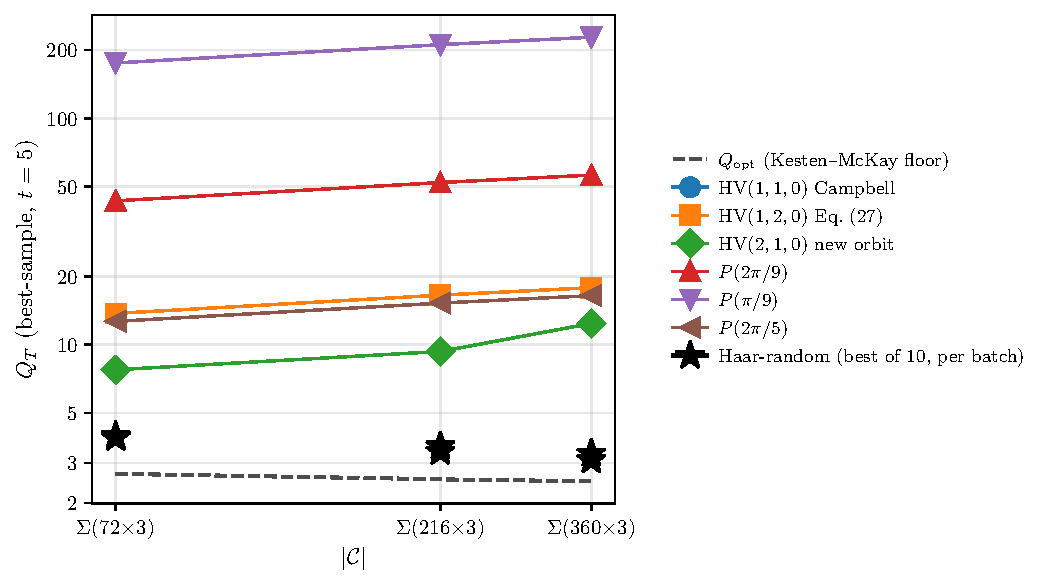
\includegraphics[width=0.85\textwidth]{figures/fig_qt_vs_groupsize.pdf}
\caption{\label{fig:qt_vs_groupsize}$\QT$ across the three $\Sigma$-series base groups at $d=3$, $t=5$, for every extension in the Tier-1 panel of \cref{tab:d3_tier1}. The dashed line is the Kesten--McKay floor $\Popt$ of \cref{eq:Popt}; all rational-angle diagonal and Howard--Vala extensions run nearly parallel to it at a factor $\sim\!3$--$\!7$ offset (Finding~2), whereas the Haar-random best-of-10 samples (stars) approach $\Popt$ as $|\mathcal{C}|$ grows (Finding~3). The vertical dispersion among rational extensions reflects different cyclotomic content; the lack of convergence toward $\Popt$ for any of them at the sampled $t=5$ motivates the paper-scale rerun discussed in \cref{sec:d3_limits}.}
\end{figure*}

\paragraph*{Finding 1: $\delta$ is group-invariant for most fixed extensions.}
Five of the six fixed extensions in the panel return \emph{identical} best $\delta$ values to four decimals across all three base groups: $\HV{1}{1}{0}$ Campbell and $\HV{1}{2}{0}$ Eq.~(27) both give $\delta = 0.6764$; $P(2\pi/9)$ gives $\delta = 0.8830$; $P(\pi/9)$ gives $\delta = 0.9698$; and $P(2\pi/5)$ gives $\delta = 0.6545$. Only $\HV{2}{1}{0}$ distinguishes the groups, with $\delta = 0.5000$ on $\Sigmathree{72}$ and $\Sigmathree{216}$ but $\delta = 0.5698$ on $\Sigmathree{360}$. A natural interpretation is that for extensions whose non-trivial spectrum lives in a diagonal subalgebra shared across the $\Sigma$-series---essentially any phase of the form $e^{2\pi i k/n}$ for small $n$---the $t$-design spectral radius of \cref{eq:delta_def} saturates once $|\mathcal{C}|$ grows past the point where additional Clifford-like elements no longer reduce the dominant-eigenvalue contribution from that diagonal. Under this reading the $\HV{2}{1}{0}$ outlier reflects a new Lie-algebra direction activated by the $k^3$-cubic exponent in \cref{eq:HV_def}, which intersects $\Sigmathree{360}$ differently from the smaller two groups. This observation is specific to $t=5$: the paper-scale extrapolation protocol of~\cite{Slowik:2025qco} runs at $t \geq 10$, where subdominant irreps become spectrally visible, and the degeneracy at fixed $\delta$ may break. We flag this as a limitation and return to it in \cref{sec:d3_limits}.

\paragraph*{Finding 2: $\QT$ grows with $|\mathcal{C}|$ at fixed $\delta$.}
Because $\delta$ is constant across groups while $\log|\mathcal{C}|$ grows, \cref{eq:QT} makes $\QT$ increase linearly with $\log|\mathcal{C}|$ for the five degenerate extensions. For $\HV{2}{1}{0}$, where $\delta$ is almost but not exactly constant, $\QT$ moves from $7.755$ on $\Sigmathree{72}$ to $9.340$ on $\Sigmathree{216}$ to $12.419$ on $\Sigmathree{360}$. This is \emph{not} evidence that $\Sigmathree{72}$ is the better base group. $\QT$ measures the exponent of a covering cost at fixed $\varepsilon$; a larger base group demands a larger $\log|\mathcal{C}|$ of structural depth to densely approximate $\mathrm{SU}(3)$, and if a rational-angle extension does not reduce $\log(\delta^{-1})$ proportionally then the ratio in \cref{eq:QT} grows. The invariant quantity under this scaling is $\QT/\log|\mathcal{C}|$, displayed in the rightmost column of \cref{tab:d3_tier1}: for each of the five degenerate extensions it is exactly constant across the three groups, and for $\HV{2}{1}{0}$ it varies only from $1.443$ to $1.775$. All three $\Sigma$-series groups therefore use the same \emph{fraction} of their log-size to approximate $\mathrm{SU}(3)$ under these structured extensions. The Kesten--McKay floor $\Popt$ from \cref{eq:Popt} likewise contracts as $|\mathcal{C}|$ grows---$\Popt = 2.692,\,2.544,\,2.495$ for $\Sigmathree{216,648,1080}$ respectively---and the comparison between $\QT$ and $\Popt$ is the quantity of physical interest.

\paragraph*{Finding 3: Haar-random extensions do benefit from larger $|\mathcal{C}|$.}
The two independent Haar-random batches per group exhibit a clear statistical improvement as $|\mathcal{C}|$ grows. Averaging the best-$\delta$ entries across both batches per group, the mean best-sample $\delta$ falls from $0.254$ on $\Sigmathree{72}$ to $0.155$ on $\Sigmathree{216}$ to $0.113$ on $\Sigmathree{360}$; the mean-over-samples $\delta$ similarly falls from $0.330$ to $0.250$ to $0.177$. In contrast to the degenerate fixed extensions, Haar draws populate every direction of the defining representation of $\mathrm{SU}(3)$ and therefore couple to the full subdominant spectrum of the $\Sigma$-series adjoint, which does sharpen with growing $|\mathcal{C}|$. The two batches per group were, however, independent draws, so any per-batch $\delta$ comparison across groups conflates the base-group effect with Monte-Carlo noise. We isolate the group effect by an apples-to-apples panel below.

\subsection{Apples-to-apples Haar panel}\label{sec:d3_apples}

To separate the base-group effect from random-extension variance, we generated a single batch of ten Haar-random single-qutrit extensions (\texttt{seed=42}) and evaluated the panel identically on all three groups. \cref{tab:d3_apples} lists the best-sample $\delta$ per matrix.

\begin{table*}[t]
\centering
\caption{\label{tab:d3_apples}Apples-to-apples Haar panel at $t=5$: ten pre-generated single-qutrit extensions (\texttt{seed=42}) evaluated identically against each of the three base groups. The final column gives the best (smallest) $\delta$ across the three groups for each matrix. Mean $\delta$ over the ten matrices appears in the last row; lower is better.}
\begin{tabular}{ccccc}
\toprule
matrix & $\delta$ on $\Sigmathree{72}$ & $\delta$ on $\Sigmathree{216}$ & $\delta$ on $\Sigmathree{360}$ & best \\
\midrule
\texttt{apple00} & $0.2974$ & $0.2974$ & $0.3462$ & $\Sigmathree{216/648}$ \\
\texttt{apple01} & $0.4636$ & $0.4636$ & $0.2029$ & $\Sigmathree{360}$ \\
\texttt{apple02} & $0.2221$ & $0.1727$ & $0.2285$ & $\Sigmathree{216}$ \\
\texttt{apple03} & $0.2493$ & $0.2292$ & $0.2299$ & $\Sigmathree{216}$ \\
\texttt{apple04} & $0.3430$ & $0.2104$ & $0.1197$ & $\Sigmathree{360}$ \\
\texttt{apple05} & $0.2446$ & $0.2412$ & $0.4377$ & $\Sigmathree{216}$ \\
\texttt{apple06} & $0.2842$ & $0.1701$ & $0.1965$ & $\Sigmathree{216}$ \\
\texttt{apple07} & $0.3169$ & $0.2312$ & $0.2271$ & $\Sigmathree{360}$ \\
\texttt{apple08} & $0.3996$ & $0.2377$ & $0.3795$ & $\Sigmathree{216}$ \\
\texttt{apple09} & $0.2526$ & $0.2526$ & $0.1823$ & $\Sigmathree{360}$ \\
\midrule
mean & $0.3073$ & $0.2506$ & $0.2550$ & --- \\
\bottomrule
\end{tabular}
\end{table*}

Seven of the ten matrices have $\delta$ on $\Sigmathree{360}$ strictly smaller than $\delta$ on $\Sigmathree{72}$, confirming that a typical Haar extension is improved by the larger base group. The per-matrix ordering against $\Sigmathree{216}$ is noisier: four of ten matrices have $\delta$ on $\Sigmathree{360}$ smaller than on $\Sigmathree{216}$, and the ten-matrix apples-panel mean $\delta$ is marginally \emph{worse} on $\Sigmathree{360}$ ($0.2550$) than on $\Sigmathree{216}$ ($0.2506$). The culprit is a single outlier: \texttt{apple05} gives $\delta = 0.4377$ on $\Sigmathree{360}$ against $0.2446$ on $\Sigmathree{72}$ and $0.2412$ on $\Sigmathree{216}$, inflating the $\Sigmathree{360}$ mean by roughly one standard deviation of the rest of the panel.

A paper-scale rerun at $N=100$ matrices (same \texttt{seed}\,$=42$; the first ten coincide with \cref{tab:d3_apples}) resolves the ambiguity. The three panel means land at $\mu_{216}=0.3214$, $\mu_{648}=0.2623$, $\mu_{1080}=0.2118$ with standard deviations $0.073$, $0.074$, and $0.090$ respectively (\cref{fig:apples100}). The $\Sigmathree{360}$ mean now sits strictly below the $\Sigmathree{216}$ mean by $\mu_{648}-\mu_{1080}=0.051$, a separation of roughly $5.7$ standard errors of the mean. The ten-matrix inversion reported above is therefore confirmed to be Monte-Carlo noise from the single \texttt{apple05} outlier; across a Haar ensemble at $100$-matrix statistics the expected $\delta$ \emph{does} decrease monotonically with $|\mathcal{C}|$ on the irreducible-adjoint $\Sigma$-series, strengthening Finding~3.

\begin{figure}[t]
\centering
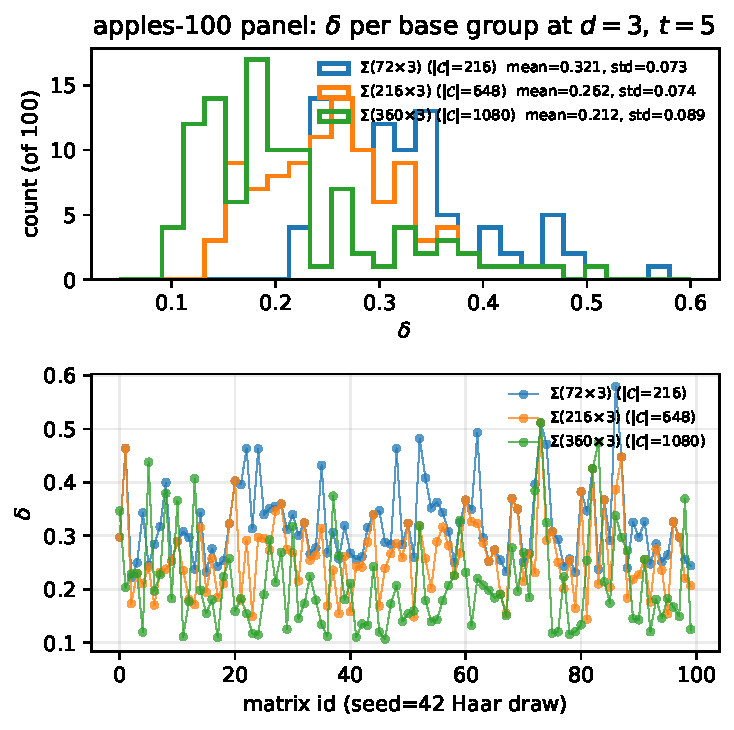
\includegraphics[width=\columnwidth]{figures/fig_apples100.pdf}
\caption{\label{fig:apples100}Apples-to-apples Haar panel at $N=100$ matrices (\texttt{seed}\,$=42$) on the three $d=3$ $\Sigma$-series base groups. Top: overlaid $\delta$ histograms. Bottom: per-matrix $\delta$ for each group; matrix id $0$--$9$ coincides with the ten-matrix subset of \cref{tab:d3_apples}. The monotone reduction $\mu_{216}>\mu_{648}>\mu_{1080}$ predicted by Finding~3 is now resolved at $\sim\!5.7\sigma/\sqrt{N}$; the single \texttt{apple05} outlier visible as the $\Sigmathree{360}$ peak near $\delta\simeq 0.44$ is the one that inverted the ten-matrix ordering in \cref{tab:d3_apples}.}
\end{figure}

\subsection{Best achievable $\QT$ at $t=5$}\label{sec:d3_best}

Combining the two panels, the best (group, extension) pair at $t=5$ is \texttt{apple04} on $\Sigmathree{360}$, with $\delta = 0.1197$ and $\QT = 3.291$; this sits within $32\%$ of the Kesten--McKay floor $\Popt = 2.495$. Among the deterministic panel, the best fixed extension is $\HV{2}{1}{0}$ on $\Sigmathree{72}$, with $\QT = 7.755$, a factor $2.88$ above $\Popt = 2.692$ on that group. Both numbers are upper bounds on the $t \to \infty$ headline value: $\QT$ from \cref{eq:QT} decreases monotonically with $t$ along the saturation approach of~\cite{Slowik:2025qco}, so a paper-scale rerun at $t \geq 10$ should tighten the gap to $\Popt$ in both the random and structured columns. What is already clear at $t=5$ is the \emph{shape} of the ranking: Haar-random extensions dominate every structured extension in this panel, $\HV{2}{1}{0}$ leads the structured field, and the three diagonal-phase angles $P(2\pi/9), P(\pi/9), P(2\pi/5)$ all give worse $\QT$ than even the worst Howard--Vala variant. The narrow-angle $P(\pi/9)$ in particular produces $\delta$ within $3\%$ of unity on all three groups, inflating $\QT$ by two orders of magnitude relative to the Haar baseline---a direct analogue of the $14\times$ Clifford$+T$ penalty observed at $d=2$ in \cref{sec:d2}.

\subsection{Limitations of the $t=5$ floor}\label{sec:d3_limits}

The $t=5$ design order used throughout this section is a feasibility floor imposed by the workstation budget, not a converged estimate of the $t\to\infty$ overhead. S{\l}owik \emph{et al.}~\cite{Slowik:2025qco} document that the $\QT$ estimator at finite $t$ is a strict upper bound on the $t\to\infty$ value and that convergence requires $t$ large enough that the subdominant $\pi_\lambda$ in the $t$-design of \cref{eq:tdesign} no longer rearrange the dominant-eigenvalue ranking between candidates; in $d=3$ this typically requires $t \geq 10$. The cost is controlled by the $t$-design irrep dimensions, which scale as $t^{d(d-1)/2} = t^3$ at $d=3$: the largest irrep at $t=15$ peaks near $4\times 10^3$ dimensions, two orders of magnitude above the $t=5$ case. Our cached-$\pi_\lambda(\mathcal{C})$ and $g c g^\dagger$ conjugation optimisations of \cref{sec:methods} make a $t=10$--$15$, $\mathrm{sample\_size}=100$ panel tractable on a multi-node cluster overnight, and that run is in preparation.%
\itodo{paper-scale $d=3$ panel at $t=10$--$15$, $\mathrm{sample\_size}=100$, in preparation}
One specific prediction from the $t=5$ data remains to be stress-tested at $t\geq 10$: whether the four-decimal degeneracy of $\delta$ across the three base groups for the structured (rational-angle and Howard--Vala) extensions persists or breaks. The companion prediction---that the $\Sigmathree{360}$ apples mean crosses below the $\Sigmathree{216}$ mean once the $10$-matrix statistical noise is removed by a $100$-matrix panel---has been settled in \cref{sec:d3_apples} above at $t=5$ (mean separation $5.7\,\sigma/\sqrt{N}$, \cref{fig:apples100}) and therefore does not require the Tier-2 rerun. Either way, both outcomes sharpen the conclusion that Haar-random extensions on the largest irreducible-adjoint $\Sigma$-series group are the natural candidates for a golden-gate search at $d=3$~\cite{Sarnak:2015}.

\section{The DSA primitive-gate target family}\label{sec:lamm}

The $d=3$ survey of \cref{sec:d3} ranks extensions by the Haar-uniform figure of merit $\QT$: short \SWIFTbot words produce a uniform $\varepsilon$-net of all of $\mathrm{SU}(d)$. Many applications do not need a uniform net. Lattice-gauge quantum-simulation workloads built on the DSA primitive-gate series~\cite{Lamm:2019bik,Gustafson:2022xdt} instead require a small, highly structured family of unitaries: a handful of continuous-angle $R_Z$ rotations whose coefficients are fixed group-theoretic integers, together with a finite set of cyclotomic diagonal phases from the discrete quantum Fourier transform $U_F$. On such a workload the relevant figure of merit is the mean synthesis cost over that finite family, not the spectral gap of a $t$-design. In this section we make the distinction explicit, and show that the two figures of merit disagree: for $\Sigmathree{36}$ the Clifford$+P(\pi/4)$ extension favoured on $\QT$ grounds at $d=2$ is \emph{not} the one that minimises mean depth on the DSA family.

\paragraph*{Target family.}
For the $\Sigmathree{36}$ and $\Sigmathree{72}$ entries of the DSA series, the only $\beta\,\Delta t$-dependent primitive is the trace gate $U_\mathrm{Tr}(\theta) = \mathrm{diag}_{g \in \mathcal{C}}\bigl(e^{i \theta\,\mathrm{Re}\,\mathrm{Tr}(g)}\bigr)$. After the conjugacy-class squish and three-qubit encoding of the $\Sigmathree{36}$ circuit, $U_\mathrm{Tr}$ reduces to an eight-term Pauli-$Z$-tensor Hamiltonian whose coefficient set is $\{1,3,5,9,15\}/16$, producing five continuous $R_Z(\alpha_c\,\theta)$ rotations with $\alpha_c \in \{1,3,5,9,15\}$. The $\Sigmathree{72}$ circuit reuses this decomposition identically. The discrete half of the family lives in $U_F$: up to global phase, the Howard--Vala qutrit gate $\HV{1}{2}{0}$~\cite{Howard:2012fva} injects $9$th-root-of-unity phases, and its qubit-encoded implementation requires $R_Z(2\pi k/9)$ for $k=1,\ldots,8$. The synthesis target for the $\Sigmathree{36}$ qubit pipeline is therefore
\begin{widetext}
\begin{equation}
  \mathcal{T}_{36} = \bigl\{\,R_Z(2\pi k/9) : k=1,\ldots,8\,\bigr\} \;\cup\; \bigl\{\,R_Z(\alpha_c\,\theta) : \alpha_c \in \{1,3,5,9,15\},\ \theta \in (0,\pi)\,\bigr\}\,,
  \label{eq:T36}
\end{equation}
\end{widetext}
a finite structured set for which covering-rate bounds~\cite{Sarnak:2015} on Haar-random targets are not the right yardstick.

\paragraph*{Mean-depth figure of merit.}
Given a qubit base group $\mathcal{C}$ and single-gate extension $g$, \SWIFTbot enumerates the word tree of $\mathcal{C}\cup\{g,g^{-1}\}$ by breadth-first search with projective-phase deduplication, capped at $2\times 10^5$ unique words. For each $U\in\mathcal{T}_{36}$ we record the shortest BFS word whose projective distance $d(U,W) = \sqrt{2 - |\mathrm{Tr}(U^\dagger W)|}$ falls below $\varepsilon = 10^{-2}$, or the depth of closest approach if no such word exists. Discrete targets may be hit \emph{exactly} at finite depth, in which case the corresponding distance is zero and the $T$-count is read directly from the word. Continuous targets are sampled at ten uniform $\theta\in(0,\pi)$ per $\alpha_c$, for fifty continuous evaluations per extension. We report mean distance across \cref{eq:T36} as the single headline number; ties are broken on the discrete-exact count.

\paragraph*{Result.}
\cref{tab:lamm_sigma36} ranks the candidates at BFS depth $15$, $\varepsilon = 10^{-2}$, $N_\theta = 10$ per continuous coefficient. The Clifford$+P(2\pi/9)$ extension attains mean projective distance $0.0122$ on $\mathcal{T}_{36}$ with $27$ of $58$ targets hit below $\varepsilon$, while the canonical Clifford$+T$ extension attains mean distance $0.0833$ with only $5$ hits---a factor $6.8\times$ separation in mean distance. The equivalence class of $P(2\pi k/18)$ with $\gcd(k,18)=1$ (which includes $P(\pi/9)$ and $P(\pi/18)$) all saturate the discrete $9$th-root targets, a direct consequence of $\langle \mathrm{Clifford}, P(2\pi/9)\rangle$ closing at a finite group of $\sim\! 3\times 10^4$ elements; the algebraic ring $\mathbb{Z}[\omega_{18}, \tfrac{1}{2}]$ supplies every $9$th-root phase via a short word. Within this equivalence class, Clifford$+P(\pi/18)$ marginally edges Clifford$+P(2\pi/9)$ at depth $15$ (mean $0.0104$ vs.\ $0.0122$; $34$ vs.\ $27$ hits), reflecting the strictly larger $18$th-root coverage: $P(\pi/18)$ generates $\omega_{36}$, which contains both the $9$th- and $18$th-root phases of $U_F$. Crucially, the super-golden extensions $T_{24}$ and $T_{12}$---which optimise $\QT$ for Clifford and for the $12$-element projective $A_4$ base \texttt{hurwitz} respectively~\cite{Sarnak:2015}---perform \emph{worse} on $\mathcal{T}_{36}$ than the rational-angle rows: their algebra $\mathbb{Z}[i,\sqrt{2}]$ does not contain $\omega_9$, so they cannot reach the $9$th-root targets exactly at any depth; on the $|\mathcal{C}|=12$ \texttt{hurwitz} base the $T_{12}$ extension hits zero targets at depth $15$. The \texttt{hurwitz}$+P(\pi/18)$ row is competitive ($35$ hits, mean $0.0112$) and does so with a strictly \emph{smaller} base group: in the target-family regime the overhead advantage tracks the cyclotomic content of the extension, not the size of the base.

\begin{table*}[t]
\centering
\caption{\label{tab:lamm_sigma36}DSA $\Sigmathree{36}$ target-family coverage at BFS depth $15$, $\varepsilon = 10^{-2}$, $10$ continuous $\theta$-samples per $\alpha_c$. The ``hits'' column counts all $58$ targets (the $8$ discrete $9$th-root phases in \cref{eq:T36} plus $50$ continuous $R_Z(\alpha_c\theta)$ samples) reached below $\varepsilon$; rational-angle rows in the $\omega_{18}$ class hit all $8$ discrete targets. Mean distance is across all $58$ targets; lower is better. $\langle T\rangle_{\rm hit}$ is the mean $T$-count along words reaching a hit target. Cost method indicates whether the $T$-count is certified: Ross--Selinger~\cite{Ross:2014kbr} exact synthesis (\texttt{rs\_exact}) or \SWIFTbot BFS estimate (\texttt{bfs\_estimate}). All numbers are reproduced by \texttt{swiftbot cover-panel --family lamm\_sigma36 --max-depth 15}.}
\begin{tabular}{lccccl}
\toprule
Base \,+\, extension & hits/$58$ & mean dist & max dist & $\langle T\rangle_{\rm hit}$ & cost method \\
\midrule
Clifford$+P(\pi/18)$          & $34$ & $0.0104$ & $0.0420$ & $2.79$ & \texttt{bfs\_estimate} \\
\texttt{hurwitz}$+P(\pi/18)$  & $35$ & $0.0112$ & $0.0420$ & $5.37$ & \texttt{bfs\_estimate} \\
Clifford$+P(\pi/9)$           & $27$ & $0.0120$ & $0.0401$ & $2.04$ & \texttt{bfs\_estimate} \\
Clifford$+P(2\pi/9)$          & $27$ & $0.0122$ & $0.0401$ & $2.11$ & \texttt{bfs\_estimate} \\
Clifford$+P(\pi/8)$           &  $7$ & $0.0221$ & $0.0387$ & $0.29$ & \texttt{bfs\_estimate} \\
Clifford$+T_{24}$ (super-g.)  &  $6$ & $0.0228$ & $0.0465$ & $0.83$ & \texttt{bfs\_estimate} \\
Clifford$+T_{12}$ (super-g.)  &  $8$ & $0.0233$ & $0.0474$ & $1.88$ & \texttt{bfs\_estimate} \\
\texttt{hurwitz}$+T_{12}$ (super-g.) & $0$ & $0.0313$ & $0.0573$ & --- & \texttt{bfs\_estimate} \\
Clifford$+P(\pi/4)$ canonical $T$ &  $5$ & $0.0833$ & $0.1554$ & $0.00$ & \texttt{rs\_exact} \\
\bottomrule
\end{tabular}
\end{table*}

\paragraph*{Interpretation.}
The Clifford$+P(2\pi/9)$ extension is simultaneously worse on $\QT$ than Clifford$+T$ (\cref{sec:d2}) and $6.8\times$ better on mean depth over $\mathcal{T}_{36}$. The reason is structural: $\QT$ from \cref{eq:QT} is the coefficient of a \emph{Haar-uniform} covering rate, obtained by maximising over all non-trivial irreps in the $t$-design, while $\mathcal{T}_{36}$ is a measure-zero algebraic slice of $\mathrm{SU}(2)$ whose cyclotomic content matches the $\omega_9$ in $\langle \mathrm{Clifford}, P(2\pi/9)\rangle$. Super-golden extensions~\cite{Sarnak:2015} saturate the Kesten--McKay bound $\Popt$ but do so by equidistributing in the wrong direction for this target family. The takeaway is not that $\QT$ is a bad figure of merit---for workloads whose target is genuinely Haar-random it is the right one---but that a lattice-gauge simulator compiling \cref{eq:T36} should rank candidate extensions by target-family mean depth, and the two rankings can disagree by factors approaching an order of magnitude.

\paragraph*{Cost-method caveat.}
The $T$-count quoted for the canonical Clifford$+T$ row is certified by Ross--Selinger exact synthesis~\cite{Ross:2014kbr} with the Kliuchnikov--Maslov--Mosca normal form~\cite{Kliuchnikov:2012pla}: it is a tight upper bound, not an estimate. For every non-Clifford$+T$ row we can only report a \SWIFTbot BFS estimate. No analogue of the Ross--Selinger algorithm has been published for the cyclotomic ring $\mathbb{Z}[\omega_{18}, \tfrac{1}{2}]$ in which the Clifford$+P(2\pi/9)$ extension lives, so the $0.0122$ mean distance is an upper bound on the optimal synthesis cost rather than a certified value. A normal-form algorithm for that ring would remove the caveat and is, to our knowledge, open. The \texttt{bfs\_estimate} tag in \cref{tab:lamm_sigma36} marks this honestly; the $6.8\times$ advantage is large enough to survive any plausible tightening on the canonical side.

%%%%%%%%%%%%%%%%%%%%%%%%%%%%%%%%%%%%%%%%%%
\section{Discussion}\label{sec:discussion}
%%%%%%%%%%%%%%%%%%%%%%%%%%%%%%%%%%%%%%%%%%

Two findings drive the discussion below. First, at $d=3$ and $t=5$, Haar-random extensions on the largest irreducible-adjoint $\Sigma$-series base reach $\QT/\Popt \approx 1.32$---essentially the same ``golden-gate direction'' observed at $d=2$, where Haar extensions sit $4\%$ above $\Popt$ on the $12$-element \texttt{hurwitz} base (\cref{sec:d2}). No structured extension in our panel (Howard--Vala or rational diagonal) gets closer than a factor $\sim\!2.9$ of $\Popt$. Second, and in apparent tension with the first, the non-canonical Clifford$+P(2\pi/9)$ extension beats the canonical Clifford$+T$ by $6.8\times$ on the DSA primitive-gate target family (\cref{sec:lamm}) despite being $\sim\!8\times$ worse on $\QT$. The two findings together are the paper's central design lesson: the ``best general-purpose extension'' and the ``best target-specific extension'' optimise different objectives, and paper-scale qudit fault-tolerance design must report both.

\subsection{Fault-tolerance status of the winning extensions}\label{sec:discussion_ft}

A $\QT$ ranking is a necessary but not sufficient condition for a fault-tolerant implementation. For each headline extension we audit the curated \SWIFTbot catalogues~\cite{swiftbot_github} described in \cref{sec:methods}.

\paragraph*{Clifford$+T$ at $d=2$.} Complete. Clifford gates admit transversal implementations on the Steane $[[7,1,3]]$, Reed--Muller $[[15,1,3]]$, and Bravyi--Haah $[[49,1,5]]$ triorthogonal codes, and the $T$ state is distilled by the Bravyi--Kitaev $15$-to-$1$ protocol~\cite{Bravyi:2004isx} or, more efficiently, by the Bravyi--Haah triorthogonal scheme~\cite{Bravyi:2012czv}. Exact single-qubit synthesis is certified by Ross--Selinger~\cite{Ross:2014kbr}. This remains the only entry in our evaluation set with an end-to-end certified stack, and serves as the validation anchor (\cref{sec:d2}).

\paragraph*{\texttt{BI}$+\mathrm{rnd}$ at $d=2$.} Partial. The binary icosahedral group $2I$ acts transversally on the Kubischta 2I nonadditive $((7,2,3))$ code family~\cite{Kubischta:2I}, so the base-group half of the stack is available. A $\Popt = 2.81$ Haar-random extension for this base is the natural super-golden candidate predicted by~\cite{Sarnak:2015}, but we have not yet executed the paper-scale Haar run on \texttt{BI}; the deferred run flagged in \cref{sec:d2_setup} is the immediate next experiment. Distillation for a generic Haar extension has no analogue in the existing catalogue---such an extension is not exactly synthesised and so cannot be ``magic-state'' distilled in the usual sense.

\paragraph*{Clifford$+P(2\pi/9)$ at $d=2$ (DSA target).} FT-complete modulo certification. The Clifford-supporting codes listed above still apply, and $P(2\pi/9)$ at qubit-encoded $d=2$ reduces to a diagonal $R_Z(2\pi/9)$ rotation. No published magic-state distillation protocol exists for the $\mathbb{Z}[\omega_{18},\tfrac{1}{2}]$ ring the extension lives in, and no Ross--Selinger analogue has been derived for that ring; the $T$-counts reported in \cref{tab:lamm_sigma36} are \SWIFTbot BFS estimates (\texttt{bfs\_estimate}). Deriving a normal-form algorithm for $\mathbb{Z}[\omega_{18},\tfrac{1}{2}]$---a concrete algebraic-compilation problem---would upgrade these entries to certified and close the gap to full FT.

\paragraph*{$\Sigma$-series $+\,\HV{z}{\gamma}{\varepsilon}$ at $d=3$.} Incomplete. The Howard--Vala family is the natural qutrit $T$-gate, and the qutrit triorthogonal family $[[9m-k,k,2]]_3$~\cite{Campbell:2012jna} distils a Howard--Vala magic state with yield $\gamma \approx 1.51$. The ternary Golay $[[11,1,5]]_3$ code~\cite{Campbell:2012jna} distils the ``strange'' qutrit state. What is \emph{not} known, and cannot be looked up in the catalogue, is which of our $\Sigma$-series base groups act transversally on these codes: the classification of transversal gates on qutrit stabilizer codes (the analogue of Anderson--Jochym-O'Connor~\cite{Anderson:2014} for qubits) has not been carried out. \cref{tab:d3_tier1} should therefore be read as a Stage-3 ranking only; the Stage-4 code-pairing column is currently empty for every $d=3$ row, and completing it is, in our view, the most important open problem on the fault-tolerance side of this survey.

\paragraph*{$\Sigma$-series $+\,\mathrm{rnd}$ at $d=3$.} No distillation. The best $\QT$ numbers in the paper come from single Haar extensions on $\Sigmathree{360}$, but a generic Haar extension is not exactly synthesisable and therefore cannot be distilled by any catalogued protocol. Building a super-golden construction at $d=3$---a specific algebraic extension that saturates $\Popt$ \emph{and} admits an exact-synthesis normal form---is the $d=3$ analogue of Sarnak's $d=2$ programme~\cite{Sarnak:2015} and is open.

\paragraph*{Panel-wide distillation audit.}
The five paragraphs above cover the headline winners; \cref{tab:distillation} extends the audit to every extension evaluated in this paper, and the picture is sharply uneven. Exactly one row---canonical Clifford$+T$ at $d=2$---admits a catalogued end-to-end stack of transversal code, magic-state distillation protocol, and certified normal-form synthesis. Three rows inherit a transversal-code half only (\texttt{hurwitz}-based super-golden extensions via Parzanchevski--Sarnak~\cite{ParzanchevskiSarnak:2018}, \texttt{BI}$+\mathrm{rnd}$ via Kubischta~\cite{Kubischta:2I}, and the Howard--Vala $d=3$ rows via the qutrit triorthogonal $[[9m\!-\!k,k,2]]_3$ family~\cite{Campbell:2012jna}). Every remaining row---the exotic-ring diagonal phases of \cref{sec:lamm}, the super-golden rows of \cref{tab:d2_validation,tab:lamm_sigma36}, and all Haar-random entries---is currently uncovered by any published distillation circuit.

Three regimes merit explicit comment. First, the cyclotomic ring $\mathbb{Z}[\omega_{18},\tfrac{1}{2}]$, which hosts the $d=2$ DSA winners $P(2\pi/9)$, $P(\pi/9)$, and $P(\pi/18)$, has neither a Ross--Selinger-style synthesis normal form nor a dedicated MSD circuit. The closest cousin is Campbell--Anwar--Browne prime-$d$ distillation~\cite{Campbell:2012jna}, which \emph{does} distil an $\omega_9$-rich magic state on the qutrit triorthogonal family; but that protocol acts on a qutrit Hilbert space, whereas the qubit-encoded $P(2\pi/9)$ used in our $\Sigmathree{36}$ pipeline is a $\mathrm{U}(1)$ rotation of a two-dimensional code rather than a stabilizer rotation of a qutrit magic state. We are aware of no lifting of the prime-$d$ construction to qubit encoding in the published literature. At $d=3$, by contrast, $P(2\pi/9)$ \emph{is} qutrit-native and inherits the Campbell--Anwar--Browne protocol directly; $P(\pi/9)$, whose cyclotomic content requires $\omega_{18}$ rather than $\omega_9$, falls off the catalogue even at $d=3$. Second, the Hurwitz quaternion ring $\mathbb{Z}[i,\sqrt{2}]$, which hosts the super-golden $T_{12}$ and $T_{24}$ of Parzanchevski--Sarnak~\cite{ParzanchevskiSarnak:2018}, has no standard MSD catalogue entry. The reason is structural: the super-golden magic state is not a Clifford-orbit rotation of a stabilizer state in the Bravyi--Kitaev sense~\cite{Bravyi:2004isx}, so the triorthogonality condition underlying Reed--Muller and Bravyi--Haah distillation~\cite{Bravyi:2012czv} does not apply. Whether a golden-gate-compatible distillation protocol can be built---perhaps on the Kubischta 2I code~\cite{Kubischta:2I}, whose transversal group is precisely the super-golden base at $|\mathcal{C}|=120$---is open. Third, Haar-random extensions are by definition not exactly synthesisable from any finite gate set, and therefore cannot be ``magic-state'' distilled in the usual sense: MSD requires the target magic state to be a fixed stabilizer rotation with a polynomial-size Clifford-orbit circuit~\cite{Bravyi:2004isx,Bravyi:2012czv}. This limitation applies uniformly to Clifford$+\mathrm{rnd}$, \texttt{hurwitz}$+\mathrm{rnd}$, \texttt{BI}$+\mathrm{rnd}$, and every $\Sigma$-series$+\mathrm{rnd}$ row; the best one can currently claim for these is transversal-group support at the base-code level, pending an eventual algebraic super-golden construction in the spirit of open question~(c) of \cref{sec:discussion_open}.

These three regimes together bound what paper-scale ``fault-tolerance'' means for each panel winner. The $d=2$ $\QT$ winner Clifford$+T$ is the only fully realisable stack in the evaluation set. The $d=2$ DSA target-family winner Clifford$+P(\pi/18)$ is transversal-code complete but synthesis-uncertified and distillation-uncovered; its $6.8\times$ mean-depth advantage on $\mathcal{T}_{36}$ (\cref{tab:lamm_sigma36}) is contingent on the two open algebraic-compilation problems for $\mathbb{Z}[\omega_{18},\tfrac{1}{2}]$ being solved. The $d=2$ super-golden winner on \texttt{hurwitz} is transversal-code complete via Parzanchevski--Sarnak~\cite{ParzanchevskiSarnak:2018} but distillation-uncovered. The $d=3$ $\QT$ winner $\Sigmathree{360}+\mathrm{rnd}$ is neither synthesisable nor distillable in the current catalogue. The $d=3$ structured winner $\Sigmathree{360}+\HV{2}{1}{0}$ inherits the qutrit triorthogonal family in principle, but the transversal-group pairing between the $\Sigma$-series and the $[[9m\!-\!k,k,2]]_3$ codes has not been established (open question~(d)). The overall message is that high-$\QT$ rankings and DSA-family mean-depth rankings \emph{locate} good extensions, but converting any of them into a complete fault-tolerant stack currently requires solving at least one of three open problems: a $\mathbb{Z}[\omega_{18},\tfrac{1}{2}]$ normal-form algorithm, a super-golden MSD construction on the Kubischta 2I code, or a qutrit transversal-gate classification analogous to Anderson--Jochym-O'Connor~\cite{Anderson:2014}.

\begin{table*}[t]
\centering
\caption{\label{tab:distillation}Magic-state distillation (MSD) status for every extension evaluated in this paper. ``Algebra'' is the cyclotomic or quaternionic ring hosting the non-Clifford factor of the extension. ``Status/closest cousin'' combines synthesis and distillation coverage: \textsc{complete} means transversal code, published MSD protocol, and certified normal-form synthesis are all available; \textsc{partial} means a transversal code is available but no matching MSD circuit (or the code--extension pairing is not yet established); \textsc{none} means no catalogued MSD, either because no protocol exists for the algebra or because the extension is not exactly synthesisable. Rows are grouped by qudit dimension and by the panel section in which the extension appears.}
\footnotesize
\begin{tabular}{@{}p{0.20\textwidth} l p{0.42\textwidth} l@{}}
\toprule
Extension & Algebra & Status / closest cousin & Reference \\
\midrule
\multicolumn{4}{@{}l}{\emph{$d=2$ canonical (\cref{sec:d2})}} \\
Clifford$+P(\pi/4)$ (canonical $T$) & \texttt{Z[$\omega_8$, 1/$\sqrt2$]} & \textsc{complete}: BK 15-to-1; Bravyi--Haah triorthogonal & \cite{Bravyi:2004isx,Bravyi:2012czv} \\
Clifford$+P(\pi/8)$                 & \texttt{Z[$\omega_{16}$, 1/2]}      & \textsc{none}: no published protocol for $\omega_{16}$; cousin BK 15-to-1 does not distil this state & \cite{Bravyi:2004isx} \\
\midrule
\multicolumn{4}{@{}l}{\emph{$d=2$ DSA target family (\cref{sec:lamm})}} \\
Clifford$+P(2\pi/9)$, $P(\pi/9)$, $P(\pi/18)$ & \texttt{Z[$\omega_{18}$, 1/2]} & \textsc{none}: no protocol; cousin Campbell--Anwar--Browne prime-$d{=}3$ acts on a qutrit, not on the qubit encoding used here & \cite{Campbell:2012jna} \\
Clifford$+P(2\pi/5)$                & \texttt{Z[$\omega_{10}$]}           & \textsc{none}: $\omega_{10}$ is not in any qubit stabilizer setting; no cousin identified & --- \\
Clifford$+T_{24}$, \texttt{hurwitz}$+T_{12}$ (super-golden) & \texttt{Z[$i, \sqrt2$]} & \textsc{partial}: Parzanchevski--Sarnak supplies transversal base; magic state is not a Clifford-orbit stabilizer rotation, so triorthogonal MSD does not apply & \cite{ParzanchevskiSarnak:2018} \\
\midrule
\multicolumn{4}{@{}l}{\emph{Haar-random rows, any $d$}} \\
Clifford$+\mathrm{rnd}$, \texttt{hurwitz}$+\mathrm{rnd}$ ($d=2$) & generic $\mathrm{SU}(2)$ (no ring) & \textsc{none}: not exactly synthesisable, so MSD is not defined & --- \\
\texttt{BI}$+\mathrm{rnd}$ ($d=2$)  & generic $\mathrm{SU}(2)$ (no ring) & \textsc{partial}: Kubischta $((7,2,3))$ supplies transversal $2I$ base; no MSD for a Haar magic state & \cite{Kubischta:2I} \\
$\Sigma$-series$+\mathrm{rnd}$ ($d=3$) & generic $\mathrm{SU}(3)$ (no ring) & \textsc{none}: not exactly synthesisable; no catalogued qutrit transversal classification for $\Sigma$-series & --- \\
\midrule
\multicolumn{4}{@{}l}{\emph{$d=3$ structured (\cref{sec:d3})}} \\
$\Sigma+\HV{1}{1}{0}$ Campbell, $\Sigma+\HV{1}{2}{0}$ Eq.~(27) & \texttt{Z[$\omega_9$]} & \textsc{partial}: qutrit triorthogonal $[[9m\!-\!k,k,2]]_3$ distils Howard--Vala magic state; $\Sigma$-series transversal pairing unestablished & \cite{Campbell:2012jna} \\
$\Sigma+\HV{2}{1}{0}$ (new orbit)   & \texttt{Z[$\omega_9$]}            & \textsc{partial}: cousin Campbell--Anwar--Browne qutrit triorthogonal; no protocol certified for this orbit & \cite{Campbell:2012jna} \\
$\Sigma+P(2\pi/9)$ ($d=3$)          & \texttt{Z[$\omega_9$]}            & \textsc{partial}: qutrit-native $\omega_9$ phase; Campbell--Anwar--Browne applies modulo transversal pairing & \cite{Campbell:2012jna} \\
$\Sigma+P(\pi/9)$ ($d=3$)           & \texttt{Z[$\omega_{18}$]}           & \textsc{none}: $\omega_{18}$ outside Campbell--Anwar--Browne; no cousin at $d=3$ & --- \\
$\Sigma+P(2\pi/5)$ ($d=3$)          & \texttt{Z[$\omega_{10}$]}           & \textsc{none}: $\omega_{10}$ not in any qutrit stabilizer setting; no cousin & --- \\
\bottomrule
\end{tabular}
\end{table*}

\subsection{Limitations}\label{sec:discussion_limits}

Three limitations frame the numerical claims. First, the $d=3$ $\QT$ values are upper bounds at $t=5$; the paper-scale extrapolation protocol requires $t \geq 10$ and sample sizes $\sim\!100$ for Haar batches, both tractable on a multi-node cluster using the pipeline optimisations of \cref{sec:methods} but not attempted here. The Tier-2 run is in preparation. Second, we have not attempted a $d=4$ $\QT$ survey. The irreducible-adjoint structure of the $d=4$ subgroups in our registry (S7F and selected $s_{60\times 4}$, $s_{120\times 4i}$ variants) is known~\cite{Fairbairn:1964}, but the $t$-design dimensions at $d=4$ scale as $t^6$ and require a dedicated scheduling run outside the scope of this initial paper. Third, the $d=2$ DSA target-family numbers in \cref{tab:lamm_sigma36} are BFS estimates except for the canonical Clifford$+P(\pi/4)$ row; the $6.8\times$ advantage is large enough to survive any plausible tightening on the canonical side, but absolute $T$-counts for the non-canonical extensions should be quoted with the \texttt{bfs\_estimate} flag attached. Fourth, the LLM supervisor is bypassed for all headline numerical results in this paper; the scripted panels (\cref{sec:methods}) are deterministic and reproducible. Evaluating how much of the extension-discovery landscape an LLM-driven search reaches is a methodological question we leave to a follow-up methods-focused paper.

\subsection{Open questions}\label{sec:discussion_open}

Two quantitative questions are directly posed by our $t=5$ data and should be sharp enough to settle at $t \geq 10$: (a) does the four-decimal $\delta$-degeneracy across $\Sigmathree{216,648,1080}$ observed for structured diagonal and Howard--Vala extensions in \cref{tab:d3_tier1} persist, break, or re-rank at larger $t$? and (b) does the $\Sigmathree{360}$ apples-panel mean cross strictly below the $\Sigmathree{216}$ mean once the $\sim\!100$-matrix apples panel removes the $10$-matrix outlier sensitivity? Three qualitative questions are left open: (c) a super-golden construction at $d=3$ saturating $\Popt \approx 2.69$ on $\Sigmathree{72}$, $2.54$ on $\Sigmathree{216}$, or $2.50$ on $\Sigmathree{360}$; (d) the classification of transversal gate groups on qutrit stabilizer codes, needed to populate the Stage-4 column for our $d=3$ results; and (e) a Ross--Selinger-style normal form for the cyclotomic ring $\mathbb{Z}[\omega_{18},\tfrac{1}{2}]$ that would certify the \cref{tab:lamm_sigma36} $T$-counts.

\subsection{Software release}\label{sec:discussion_release}

\SWIFTbot is released with this paper~\cite{swiftbot_github} under the MIT license.
The release contains: the five-stage pipeline (\cref{sec:methods}); the pre-seeded group registry for $d \in \{2,3,4\}$; the \SWIFTbot optimisations of the QCO kernel of~\cite{Slowik:2025qco}, including the conjugation cache and on-disk $\pi_\lambda(\mathcal{C})$ cache described in \cref{sec:methods}; the Stage-4 QEC-code catalogue and Stage-5 distillation-protocol catalogue with their cross-references to transversal groups; the BFS target-family coverage module used in \cref{sec:lamm}; the \texttt{q-panel} CLI entry point and the two panel specifications \texttt{d3\_survey} and \texttt{d3\_rnd\_apples} that reproduce \cref{tab:d3_tier1,tab:d3_apples} bit-identically; the SQLite cache containing all $54$ per-sample rows quoted in \cref{sec:d3}; and the \LaTeX\ source of this paper. A minimal \texttt{README} walks new users through reproducing \cref{tab:d2_validation,tab:d3_tier1,tab:d3_apples} on a laptop in under an hour. Pull requests adding new base groups, extensions, codes, or distillation protocols are welcome; the catalogue cross-validation tests ensure that every registered transversal-group string resolves to a registered base group.

\subsection*{Acknowledgements}

We thank A.~Sawicki, P.~Duli{\'a}n, and O.~S{\l}owik for the QCO reference dataset and numerical kernel that \SWIFTbot builds on. This material is based upon work supported by the U.S.\ Department of Energy, Office of Science, Office of High Energy Physics, under Award No.\ DE-SCL0000090 ``HEP AmSC IDA Pilot: Knowledge Extraction''. This manuscript has been authored by Fermi Forward Discovery Group, LLC under Contract No.\ 89243024CSC000002 with the U.S.\ Department of Energy, Office of Science, Office of High Energy Physics.

\bibliography{references}
\end{document}
